\documentclass{article}
%packages
\usepackage{graphicx}
\usepackage{epigraph}
\usepackage[T1]{fontenc}
\usepackage[utf8]{luainputenc}
\usepackage[compat=1.1.0]{tikz-feynman}
\usepackage{amsthm}
\usepackage{amsmath}
\usepackage[font={small,it}]{caption}
%\usepackage[a5paper, total={4.5in, 7in}]{geometry} %formato libro piccolo
\usepackage[a4paper, total={7.5in, 10.35in}]{geometry} %formato libro A4
\usepackage{hyperref}
\usepackage{color,soul}
\usepackage{amsfonts}
\usepackage{amssymb}
\usepackage{imakeidx}
\usepackage{enumerate}
\usepackage{cancel}
\usepackage{physics}
\makeindex[options=-s mystyle.ist]
\usepackage{simplewick}
%\usepackage{empheq}
\usepackage{tikz}
\usepackage{graphicx}
\usepackage{braket}
\graphicspath{ {./images/} }
\usepackage{titlesec}
\usepackage{fancyhdr}
\usepackage{subcaption}
\usepackage{kpfonts}
\usepackage{listings}
\usepackage{xcolor}
% bibliography
\usepackage[
    backend=biber,
    style=alphabetic,
    sorting=ynt
]{biblatex}
\addbibresource{bibliography/bibliography.bib}
% algorithm
\usepackage{algorithm}
\usepackage[noend]{algpseudocode}%
% multicolumns
\usepackage{multicol}

\title{Motorize 1980 dad's telescope}

\author{Sebastiano Cocchi \& Stefano Cocchi}

\date{\today}

\begin{document}
    
    \maketitle

    \begin{abstract}
        A 1980 (old and dusty) equatorial telescope is converted to an up-to-date, motorized and computer-connected telescope.
        We, me and my father, illustrate all the transformation steps from an old, dusty and unused telescope into an optimal tool for astrophotography.
    \end{abstract}

    \tableofcontents

    \begin{multicols}{2}
        \section{Telescope Description}
        The starting point of the project is of course the telescope.
        In our garage, for many years, a 1980 Urania telescope has eaten a lot of dust.
        The telescope's mirror resent of years in humidity and temperature jumps in the garage.
        In the beginning, we have cleaned the silvered-mirror with soap and water, but the silver seemed to be a bit compromised.
        We do not talk long about this telescope, since we have soon substituted it with a brand-new Skywatcher Quattro.
        The latter is placed on the Urania mount, since it is still a nice mount and, in our advice, has still not surpassed robustness.
        Indeed, the mount is a very heavy (telescope and mount totally weight 20kg!) equatorial and motorized (still works!) mount.
        
        For our money, but most importantly for our fun and entertainment, we decided to modernize our old telescope.

        \subsection{Urania telescope}
        We briefly add the specifics of the old Urania telescope, as a sort of respect for many years of honorable work before the deep dark in the garage.

        The telescope is a Urania C.R.T. NX 155, as the one in figure \ref{fig:urania_telescope_mount}.
        \\
        \begin{minipage}{0.5\textwidth}
            \centering
            \begin{tabular}{c|c}
                Specific name & value \\
                \hline
                type & reflector \\
                technique & Newton  \\
                material & PVC  \\
                weight (kg) & 10 \\
                aperture (mm) & 155 \\
                focal length (mm) & 1000 \\
                focal & f/6.5 \\
                resolution power & 0.8 \\
                limit magnitude value (mag) & 13.6 \\
                Mirror Treatment & Silica monoxide \\
                \hline
            \end{tabular}
            \captionof{table}{Urania C.R.T. NX 155 specifics.}
        \end{minipage}
        \\
        \begin{minipage}{0.5\textwidth}
            \centering
            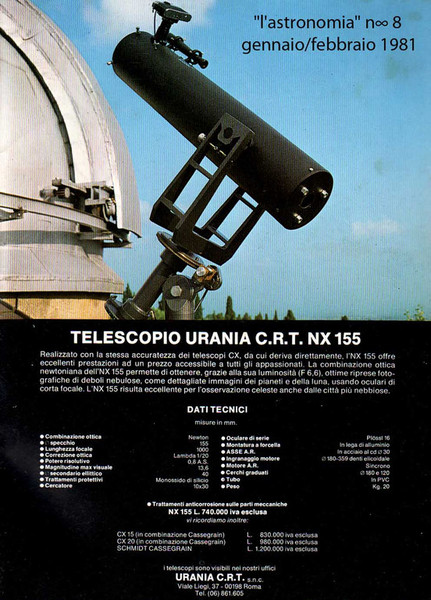
\includegraphics[scale=0.4]{images/urania_upper.jpg}
            \captionof{figure}{Urania telescope and mount.}
            \label{fig:urania_telescope_mount}
        \end{minipage}

        \subsection{Skywatcher 8P Quattro telescope}
        Skywatcher 8P Quattro Newtonian (figure \ref{fig:skywatcher_telescope_mount}) telescope offer an optimal astrophotography performance.
        For this reason we have decided to substitute the Urania telescope with this brand-new Skywatcher telescope.
        \\
        \begin{minipage}{0.5\textwidth}
            \centering
            \begin{tabular}{c|c}
                Specific name & value \\
                \hline
                type & reflector \\
                technique & Newton  \\
                material & Carbon  \\
                weight (kg) & 8.0 \\
                aperture (mm) & 200 \\
                focal length (mm) & 800 \\
                focal & f/4 \\
                resolution power & 0.58 \\
                limit magnitude (mag) & 13.3 \\
                collect light & 820 \\
                magnification & 400 \\
                Mirror Treatment & Aluminum Coating \\
                Focuser & Crayford dual-speed 50.8/31.8 \\
                \hline
            \end{tabular}
            \captionof{table}{Skywatcher 8P Quattro}
        \end{minipage}
        \\
        \\
        \begin{minipage}{0.5\textwidth}
            \centering
            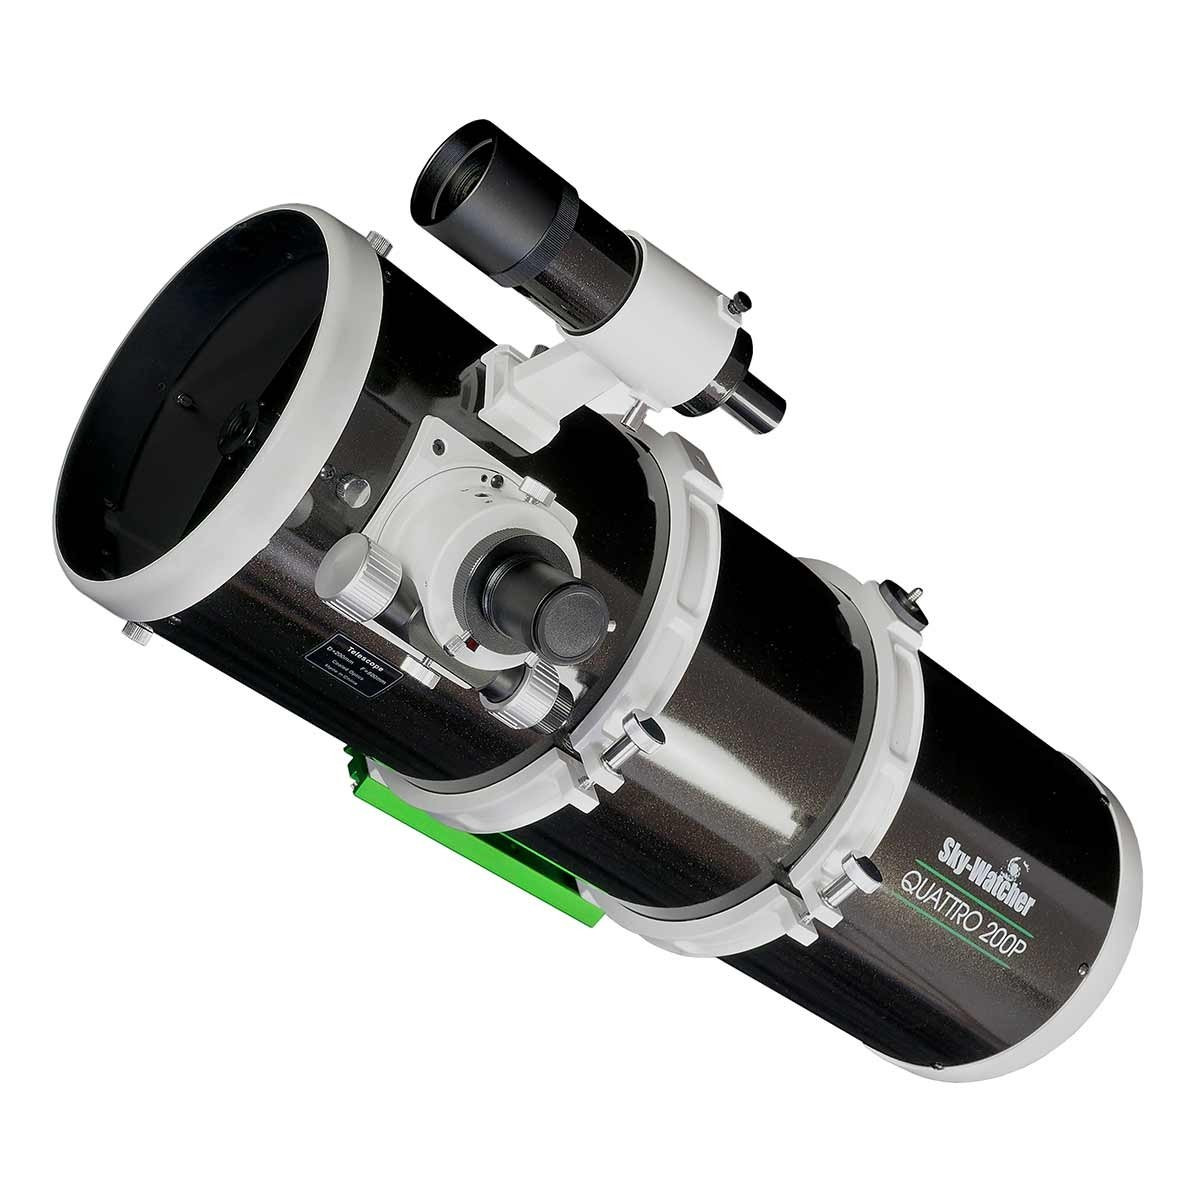
\includegraphics[scale=0.2]{images/newton-quattro-200-sky-watcher.jpg}
            \captionof{figure}{Skywatcher Quattro telescope.}
            \label{fig:skywatcher_telescope_mount}
        \end{minipage}

        \subsection{Telescope's mount}
        The telescope is place onto an aeronautic Aluminum tripod equatorial mount.
        \\
        \begin{minipage}{.5\textwidth}
            \centering
            \begin{tabular}{cc}
                Specific & value \\
                \hline
                weight (kg) & \\
                type & fork \\
                material & Aluminum alloy \\
                RA axis diameter (mm) & 30 \\
                RA axis material & cadmium steel \\
                RA motor & 3W synchronous \\
                \hline
            \end{tabular}
            \captionof{table}{Urania's mount specifics.}
            1label{tab:mount}
        \end{minipage}

        Starting from the bottom, from a central post, three pods of 30cm depart from the center. Each one has a wheel which permits the structure to move freely and then to fix the position using stops.
        The central post terminates with the second post with an inclination equal to the Earth's ecliptic \(23.43^{\circ} = 23^{\circ} 26'\).

        This axis must be aligned with the Polar star (labelling the North).
        In this way, a 3W electric motor can follow the sky movement.

        Departing from this second axis, a two-arms fork is free to rotate around two degrees-of-freedom defining the right ascension (RA) and the declination (DEG).
        The two arms are separated by the distance \(d = 15\)mm which is the Urania telescope aperture.

        \section{Telescope substitution: from Urania's tube to Skywatcher's tube}
        Passing from the Urania telescope to Skywatcher telescope we have faced the problem of how to insert the latter in the telescope mount.
        Indeed, since Skywatcher's telescope diameter is 200mm it does not fit inside the mount fork.

        Our solution is to insert a seat in which to place the telescope.
        The barycenter of the telescope is not centered with the DEC axis, thus we have settled a post capable of holding weights to balance the forces.
        See figure \ref{fig:piastra_DEC} and \ref{fig:piastra_particular}.
        \\
        \begin{minipage}{0.5\textwidth}
            \centering
            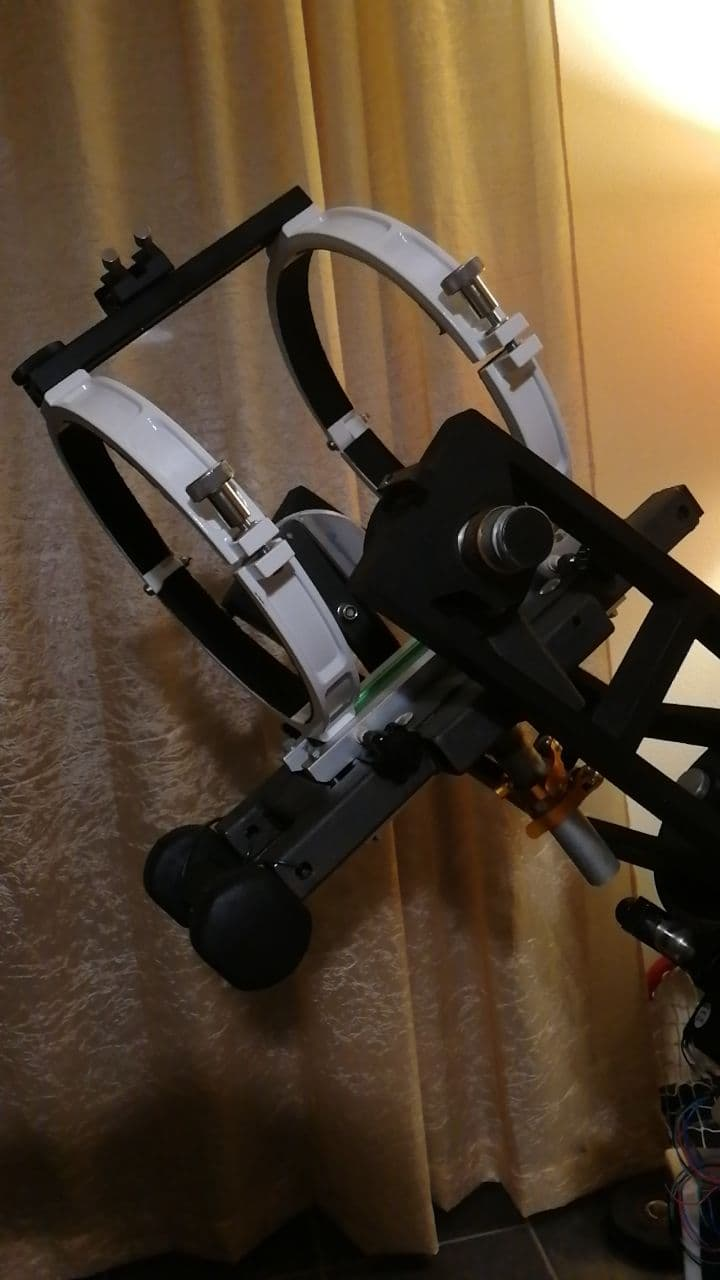
\includegraphics[scale=0.5]{images/DEC_sede.jpg}
            \captionof{figure}{The mechanism built to insert Skywatcher's telescope into the Urania robust mount.}
            \label{fig:piastra_DEC}
        \end{minipage}
        \\
        \begin{minipage}
            {0.5\textwidth}
            \centering
            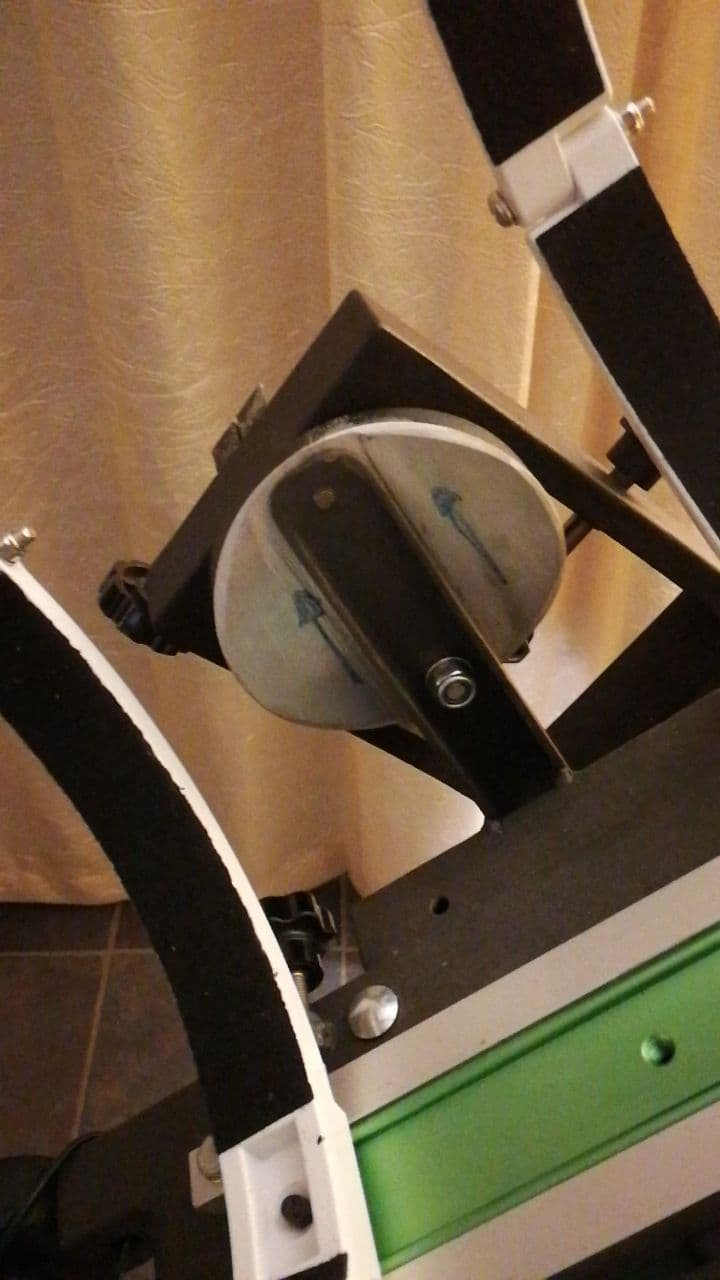
\includegraphics[scale=0.5]{images/DEC_piastra.jpg}
            \captionof{figure}{Particular of the plate.}
            \label{fig:piastra_particular}
        \end{minipage}
        \\
        The scheme with distances is visible in figure \ref{fig:DEC_piastra_dimensioni}.
        \\
        \begin{minipage}
            {0.5\textwidth}
            \centering
            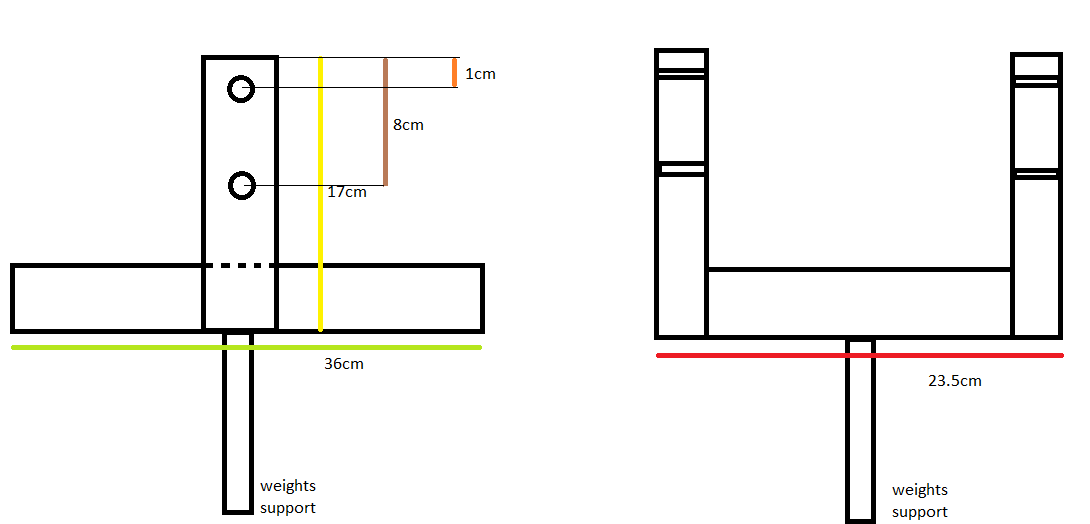
\includegraphics[scale=0.75]{images/DEC_piastra_dimensioni.png}
            \captionof{figure}{Schematic view of the telescope mount insertion. This represents only the structure we have build with some metal squared bars upon which the two white loops (which hold the telescope tube) are fixed and are not illustrated in this scheme. The two holes in each arm serve to fix the structure on the mount. }
            \label{fig:DEC_piastra_dimensioni}
        \end{minipage}

        \section{Motorization: the mechanics}
        The motorization of the telescope passes through two mechanics adjustments:
        \begin{enumerate}
            \item motorize the RA movement, exploiting the native mechanism tracker mechanism;
            \item motorize the DEC movement, which natively has no gears.
        \end{enumerate}

        \subsection{RA motorization}
        The telescope's mount has already a tracking mechanism motorized by a 3W continuous motor.
        So, in principle, it is only a matter of substitute this old motor, with a new programmable stepper motor.

        The gears are composed by:
        \begin{itemize}
            \item a 360 teeth gear (1 tooth for each degree, fantastic);
            \item an endless screw mounted on a shaft.
        \end{itemize}
        Using this structure, for a continuous sky tracking, the elder motor would complete a round of the endless screw in 4 minutes.
        Thus, this mechanism rotates the mount with the velocity of a degree in 4 minutes (which is the velocity of the sky moving away in the night).

        We have reduced the ratio by a third adding two other gears (see figure \ref{fig:RA_mechanization}): 60 teeth gear positioned in the shaft and a 20 teeth gear on the motor shaft.
        \\
        \begin{minipage}{.5\textwidth}
            \centering
            \begin{tabular}{cc|c}
                ratio gear 1 & ratio gear 2 & total ratio \\
                \hline
                1/360 & 1/3 & 1/1080 \\
                \hline
            \end{tabular}
            \captionof{table}{Total reduction of RA mechanization.}
            \label{tab:RA_mechanization}
        \end{minipage}
        \\
        \begin{minipage}{.5\textwidth}
            \centering
            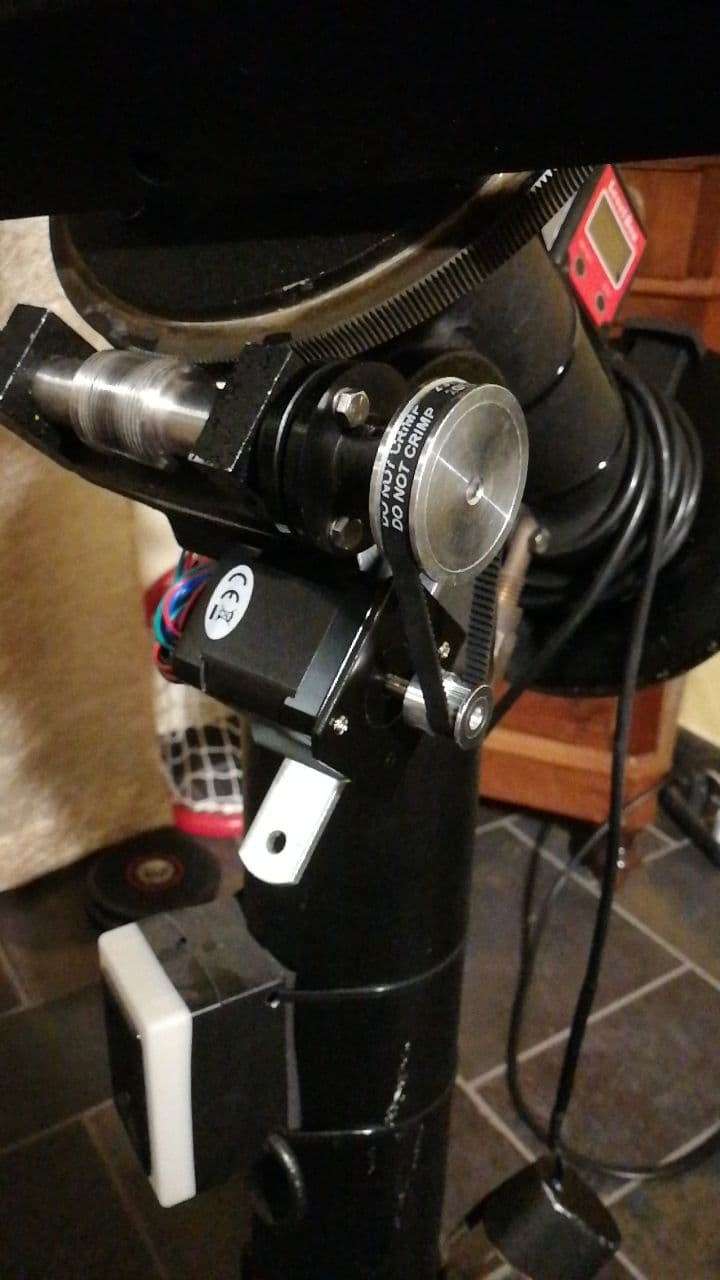
\includegraphics[scale=0.5]{images/RA_motorization.jpg}  
            \captionof{figure}{Nema 17 stepper motor and gear adjustment.}
            \label{fig:RA_mechanization}         
        \end{minipage}

        \subsection{DEC motorization}
        \hl{ancora da pensare}

        \section{Motorization: the software}
        \subsection{The Arduino experience}
        We decide to write this section more as an advertisement to not follow this way than for other purposes.

        The first, natural, approach was to try to use some at-home-technology.
        Alone on a shelf, an Arduino UNO R3 card was waiting to take part of another project with some friends: a 28BYJ-48 stepper motor and colorful cables.
        What a better occasion to be mounted on the telescope in turns of the 3W motor?

        With some fortunate events, the stepper motor is adapted to the telescope's rotating shaft.
        Was it good as a tracker motor with a constant motion?
        The answer is no.
        Indeed, some tests revealed bad performances like the inconstant rotation and several stops due to lack of robustness of the motor.
        This result was easily supposed from the beginning, but this try was costs-less, \(i.e.\) free since all the components were at home.
        Indeed, citing Wayne Gretsky:
        \begin{quote}
            "you miss one hundred percent of the shots you don't take",
        \end{quote}
        so it was a matter of must-a-do proof.
        It also gave us the opportunity to face some \textit{engineering} problems.

        The 28BYJ-48 stepper motor, sadly, returns onto its shelf as, shortly after, would do the Arduino UNO card.

        \subsection{RA stepper motor}
        In little internet journey we found a new stepper motor with a nema 17 standard; its characteristics are in table \ref{tab:nema_17_specifics}.
        \begin{minipage}{0.5\textwidth}
            \centering
            \begin{tabular}{cc}
                \textbf{Electronics}&\\
                \hline
                Manufacturer code & 17HM15-0904S\\
                Engine type & bipolar\\
                Pitch angle (deg) & 0.9 \\
                Sealing pair (Ncm)& 36\\
                Rated current/phase (A) & 0.9\\
                Phase resistance (Ohm)& 60\\
                Voltage (V)& 5.4\\
                Inductance (mH)& 12 \(\pm\) 20\% (1 kHz)\\
                &\\
                \textbf{Physical specifications}&\\
                \hline
                Frame dimensions (mm\(^2\))& 42x42 \\
                Body length (mm)& 40 \\
                Shaft diameter (mm)& 5 \\
                Stem length (mm)& 22 \\
                D-cut length (mm)& 15 \\
                Number of leds & 4\\
                Lead number (mm)& 300 \\
                Weight & 280 g\\
                \hline
            \end{tabular}
            \captionof{table}{Nema 17 stepper motor specifics.}
            \label{tab:nema_17_specifics}
        \end{minipage}

        \section{ESP32}
        After buying the new stepper motor, on the internet we have found good impressions on the ESP32 microcontroller.
        ESP32 is a series of low-cost, low-power system on a chip microcontrollers with integrated Wi-Fi and dual-mode Bluetooth.
        We've bought it. Also Arduino returned on the self with its friends.

        \section{Optics list}

    \end{multicols}
\end{document}